\chapter{Xây dựng hệ thống phân loại tự động}
\paragraph{Giới thiệu} Qua các chương trước, chúng em đã trình bày các cơ sở lý thuyết nghiên cứu được từ Semantic Web, Ontology Web Language và giới thiệu khái quát về OWL-API, Vaadin Framework - 2 công cụ nền tảng chính xây dựng nên ứng dụng phát triển ontology trên Web và từ đó sử dụng chúng để phân loại, chúng em tạm đặt tên là UIT-OWL Editor. Trong chương này, chúng em sẽ trình bày một cách chi tiết nhất có thể về quá trình xây dựng và phát triển nên ứng dụng hay hệ thống này.
\section{UI của ứng dụng}

\subsection{OWLEditorUI}
Lớp \textit{OWLEditorUI} thừa kế từ lớp \textit{UI} của Vaadin chính là User Interface của toàn bộ ứng dụng, hoạt động của lớp này tương tự miêu tả của chúng em ở chương trước khi giới thiệu về Vaadin. Chức năng của lớp này gồm:
\begin{enumerate}
	\item Chứa 2 View chính là EntryView và MainView.
	\item Cung cấp đối tượng \textit{OWLEditorKit} cho các UI Component sử dụng qua getter \textit{OWLEditorUI.getEditorKit} nhằm đảm bảo \textit{OWLEditorKit} chỉ khởi tạo 1 lần và chỉ liên kết đến 1 UI là \textit{OWLEditorUI}.
	\item Cung cấp đối tượng \textit{HttpSession} cho các UI Component qua getter \textit{OWLEditorUI .getHttpSession}.
	\item Cung cấp cơ chế reload để nạp ontology mới qua hàm \textit{updateContent}
	\item Cung cấp cơ chế xử lý sự kiện \textit{OWLEditorEventBus} nhằm xử lý các sự kiện cho ứng dụng.
\end{enumerate}
%
\subsection{Các view chính}
Ứng dụng UIT-OWLEditor chỉ gồm 2 View chính: 
\begin{description}
\item[Entry View] tương đương với lớp \textit{vn.edu.uit.owleditor.EntryView} trong mã nguồn, là nơi nhận đầu vào URL của file OWL2 Ontology hoặc tải lên (upload) file OWL2 Ontology với các định dạng được trình bày trong chương 2. Khi load được ontology \textit{EntryView} sẽ lưu đối tượng \textit{OWLEditorKit} lại trong \textit{HttpSession} phòng trường hợp người dùng mất kết nối với ứng dụng.
\begin{figure}[h!]
	\centering
	\frame{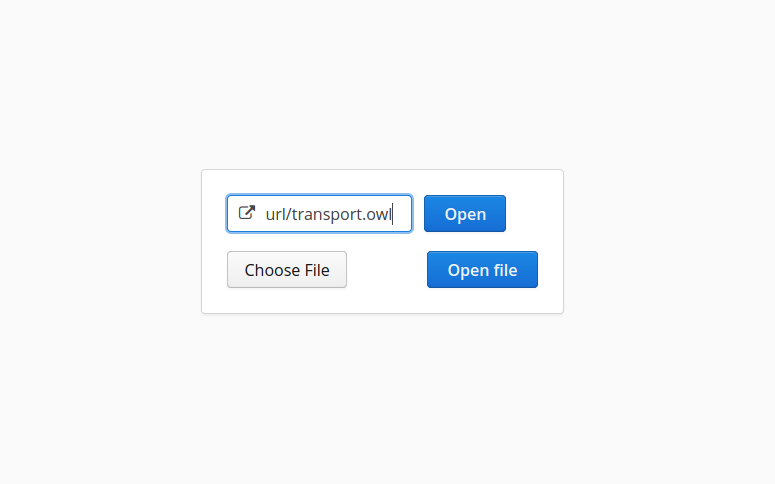
\includegraphics[width=100mm]{Figures/owleditor_entryview.png}}
	\caption{EntryView của UIT-OWL Editor\label{overflow}}
\end{figure}
\item[Main View] tương đướng với lớp \textit{vn.edu.uit.owleditor.MainView} trong mã nguồn, là giao diện chính của ứng dụng UIT-OWL Editor.
\end{description}
%
\subsection{Các tabsheet trong Main View}
Trong \textbf{MainView} sử dụng Component TabSheet các chứa các Tab tương ứng với các thực thể trong OWL2 Ontology, riêng 2 Tab cuối dùng cho việc demo tính năng phân loại là Tab Demo và Tab cuối cùng là Diagram dùng để vẽ các diagram, đồ thị phân cấp các đối tượng trong OWL 2 Ontology.

% Class Tab
\subsubsection{Tab Classes} 
\begin{figure}[h!]
	\centering
	\frame{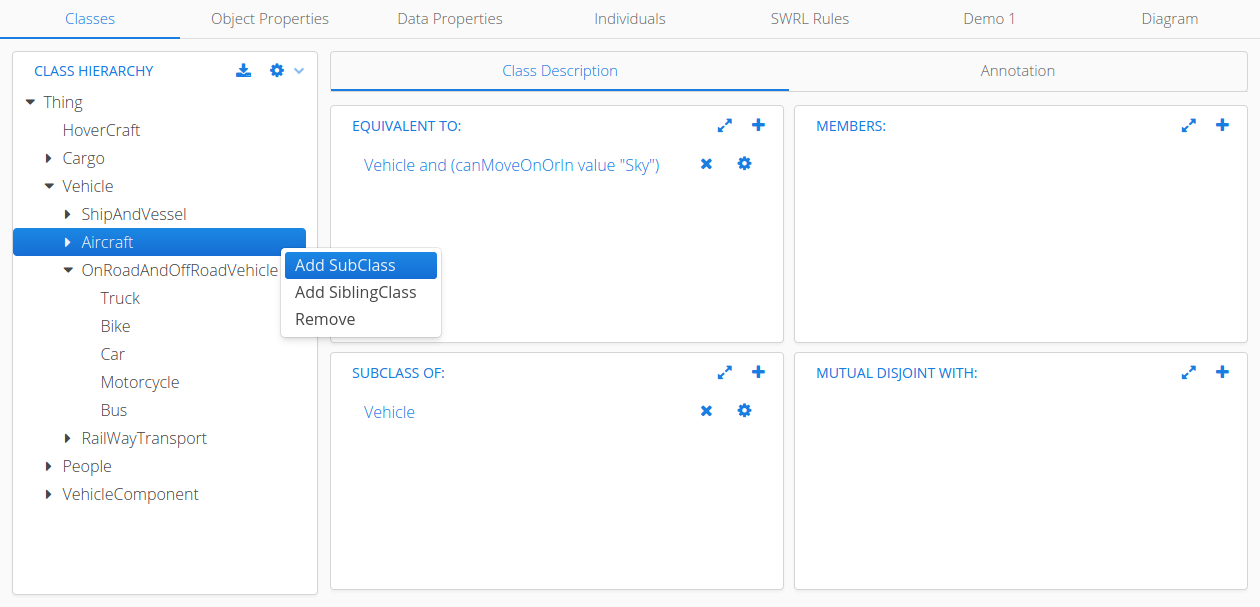
\includegraphics[width=145mm]{Figures/owleditor_classSheet.png}}
	\caption{Class Tab trong UIT-OWL Editor\label{overflow}}
\end{figure}
Tương ứng với lớp \verb|vn.edu.uit.owleditor.view.ClassesSheet| trong mã nguồn. Giao diện sử dụng HorizontalLayout của Vaadin gồm :
\begin{enumerate}
\item Panel bên trái là ClassHierachicalPanel có một cấu trúc dạng cây với các node chính là các lớp nằm trong OWL2 Ontology, với các chức năng thêm/xóa Sub/Sibling Class.
\item Các panel nhỏ bên phải được chứa trong lớp ClassExpressionPanelContainer, mỗ panel thể hiện một mô tả tương ứng với tên của panel đó.
\end{enumerate}	

% Object Property Tab
\subsubsection{Tab Object Properties}  
\begin{figure}[h!]
	\centering
	\frame{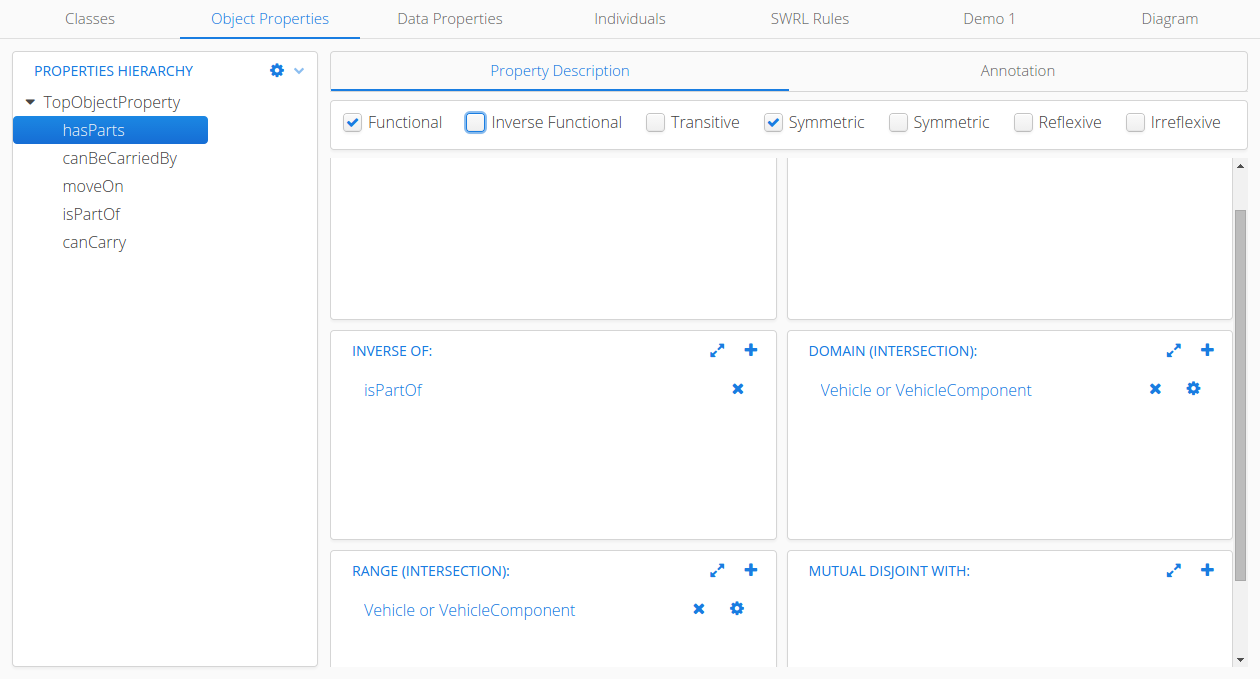
\includegraphics[width=145mm]{Figures/owleditor_opSheet.png}}
	\caption{Object Properties Tab trong UIT-OWL Editor\label{overflow}}
\end{figure}
Tương ứng với lớp \verb|vn.edu.uit.owleditor.view.ObjectPropertiesSheet| trong mã nguồn. Giao diện sử dụng HorizontalLayout của Vaadin gồm :
\begin{enumerate}
\item Panel bên trái là ObjectPropertyHierachicalPanel có một cấu trúc dạng cây với các node đại diện cho các thuộc tính đối tượng trong OWL2 Ontology, với các chức năng thêm/xóa Sibling/Sub Object Property.
\item Một dãy các \textit{CheckBox} dùng để thêm/xóa với các phát biểu trong mục 3.3.6.2 liên quan đến thuộc tính đối tượng được chọn bên trong cấu trúc cây ở bên phải.
\item Các panel nhỏ bên phải được chứa trong lớp ObjectPropertyExpressionPanelContainer, mỗ panel thể hiện một mô tả tương ứng với tên của panel đó về thuộc tính đối tượng đang được chọn trên cấu trúc cây.
\end{enumerate}	

% Data Property Tab
\subsubsection{Tab Data Properties}
\begin{figure}[h!]
	\centering
	\frame{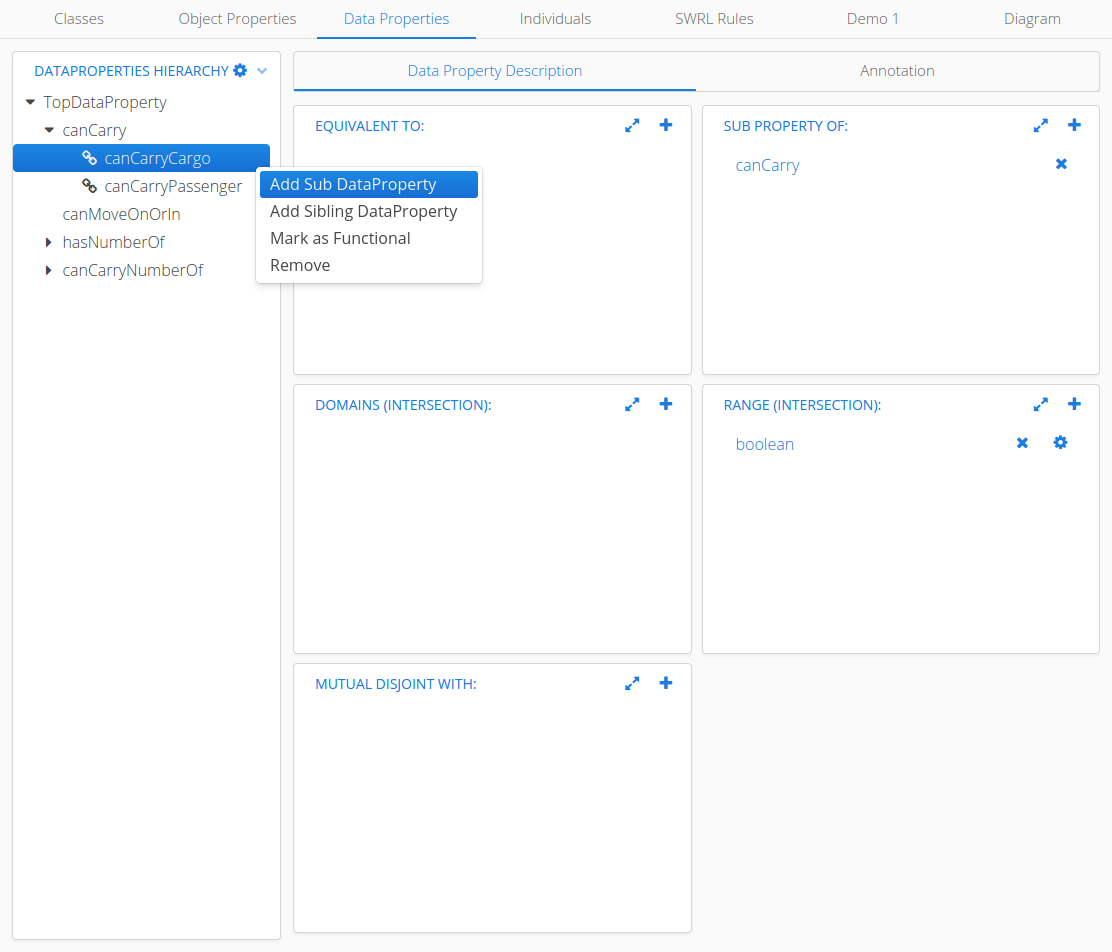
\includegraphics[width=145mm]{Figures/owleditor_dpSheet.png}}
	\caption{Data Properties Tab trong UIT-OWL Editor\label{overflow}}
\end{figure}
Tương ứng với lớp \verb|vn.edu.uit.owleditor.view.DataPropertiesSheet| trong mã nguồn. Các thành phần của tab này gồm:
\begin{enumerate}
\item Panel bên phải là DataPropertyHierachicalPanel có một cấu trúc dạng cây với các node đại diện cho các thuộc tính dữ liệu trong OWL2 Ontology, ngoài chức năng thêm/xóa Sibling/Sub DataProperty còn có tính năng thêm/xóa phát biểu FunctionalDataProperty (những thuộc tính nào có icon phía có nghĩa là có phát biểu FunctionalDataProperty về thuộc tính đó trong ontology).
\item Các panel nhỏ bên phải được chứa trong lớp ObjectPropertyExpressionPanelContainer, mỗi panel thể hiện một mô tả tương ứng với tên của panel đó về thuộc tính dữ liệu đang được chọn bên cấu trúc cây.
\end{enumerate}	

% Individual Tab
\subsubsection{Tab Individual}
\begin{figure}[h!]
	\centering
	\frame{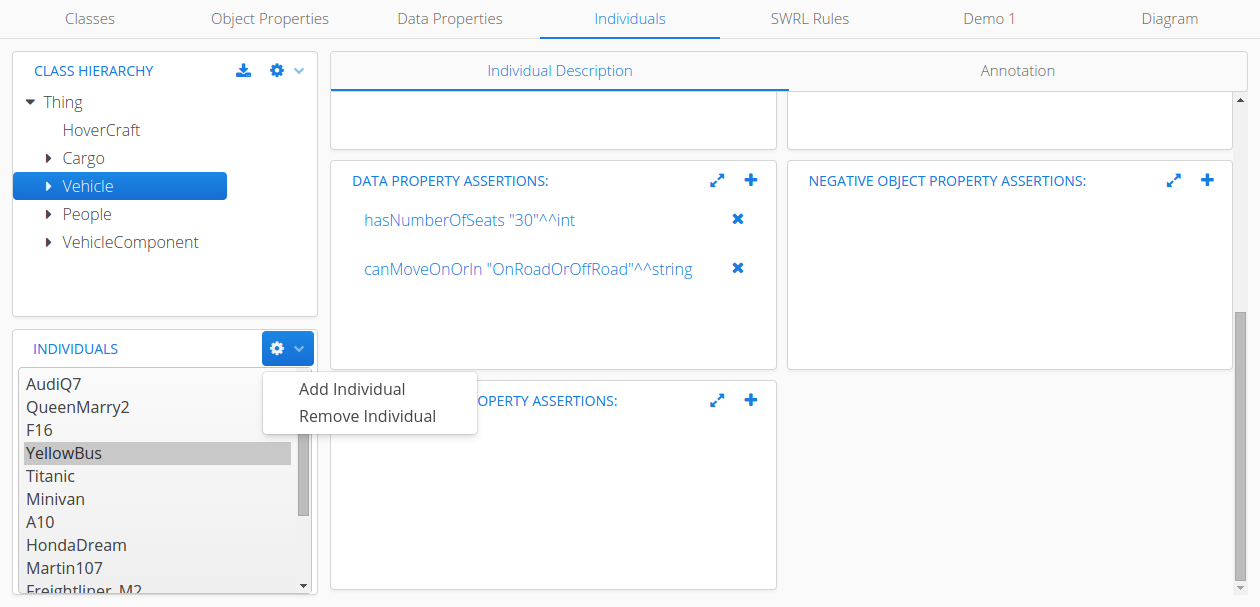
\includegraphics[width=145mm]{Figures/owleditor_individualSheet.png}}
	\caption{Individuals Tab trong UIT-OWL Editor\label{overflow}}
\end{figure}
Tương ứng với lớp \verb|vn.edu.uit.owleditor.view.IndividualsSheet| trong mã nguồn. Các thành phần của tab này gồm:
\begin{enumerate}
	\item Panel bên trái phía trên là ClassHierachicalPanel có một cấu trúc dạng cây với các node chính là các lớp nằm trong OWL2 Ontology, với các chức năng thêm/xóa Sub/Sibling Class. Khi chọn một lớp ở đây thì ListSelect ở bên dưới sẽ hiển thị một danh sách cá thể thuộc lớp này.
	\item Panel bên trái phía dưới là IndividualList hiển thị một danh sách gồm các cá thể thuộc lớp được chọn ở trên, có các tính năng thêm/xóa cá thể.
	\item Các panel bên phải là những panel biểu diễn các phát biểu assertion về cá thể. Tên panel cũng tương ứng với tên phát biểu trong OWL2.
\end{enumerate}

% SWRL Tab
\subsubsection{Tab SWRL}
\begin{figure}[h!]
	\centering
	\frame{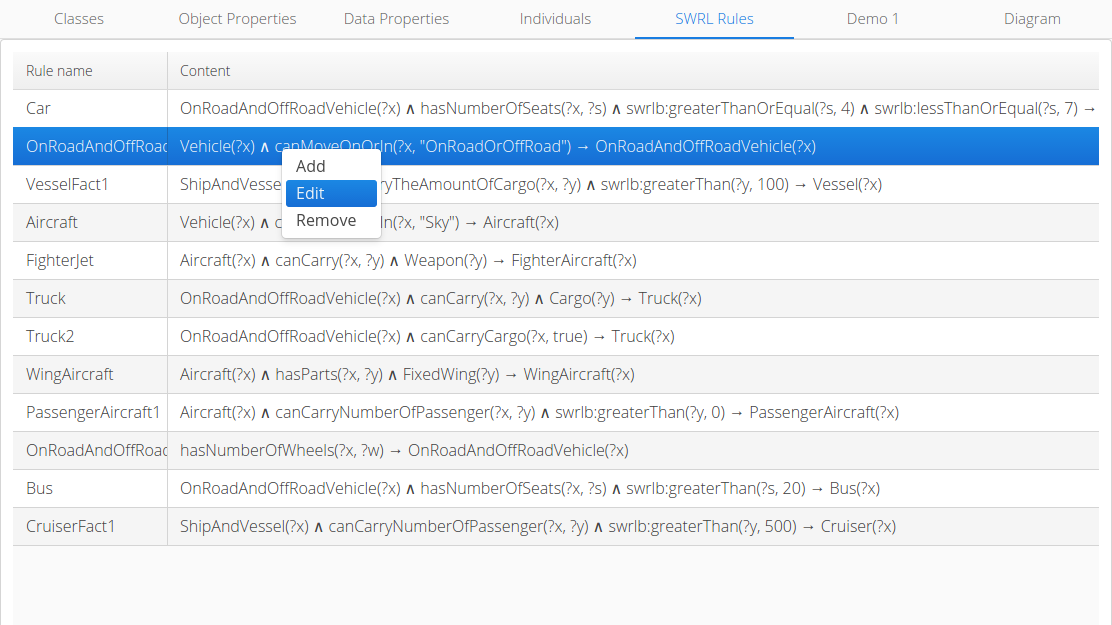
\includegraphics[width=145mm]{Figures/owleditor_swrlSheet.png}}
	\caption{SWRL Rule Tab trong UIT-OWL Editor\label{overflow}}
\end{figure}
Tương ứng với lớp \verb|vn.edu.uit.owleditor.view.RuleSheet| trong mã nguồn. Tab này chỉ gồm một thành phần chính là một Table chứa các SWRL trong tài liệu OWL 2 Ontology. Khi right-click sẽ có các chức năng thêm/xóa/sửa rule được chọn.

\subsubsection{Tab Diagram}
\begin{figure}[h!]
	\centering
	\frame{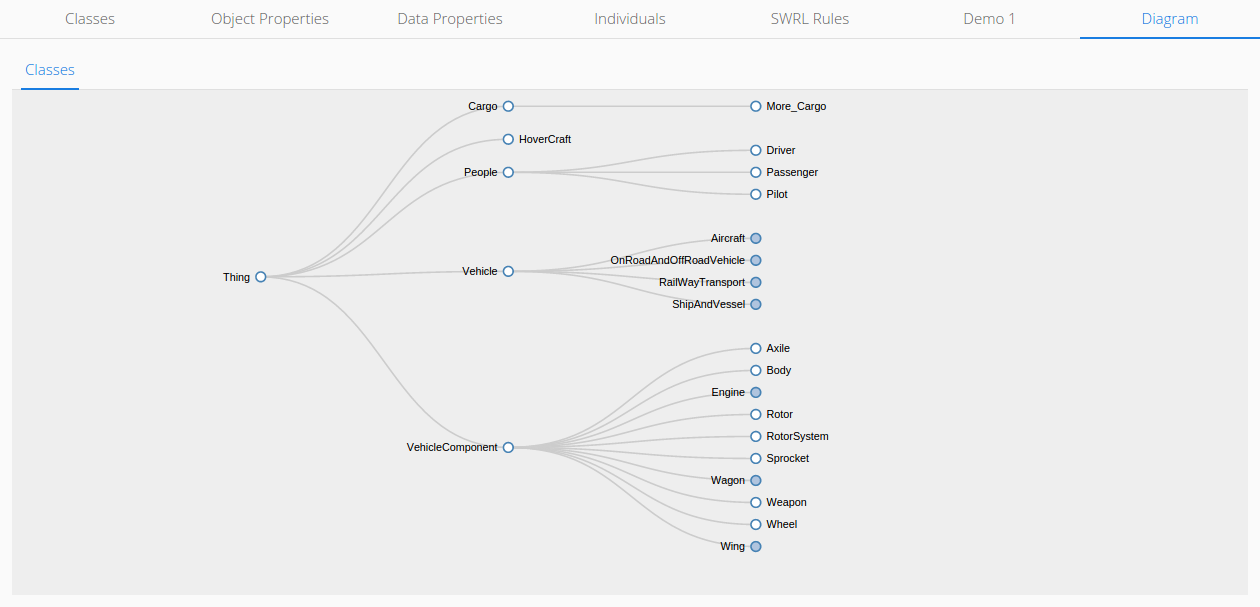
\includegraphics[width=145mm]{Figures/owleditor_diagramSheet.png}}
	\caption{Diagram Tab trong UIT-OWL Editor\label{overflow}}
\end{figure}
Diagram Tab gồm các đồ thị, sơ đồ về biểu diễn cấu trúc phân cáp của lớp bằng các đồ thị từ thư viện D3js.

% Demo Sheet
\subsubsection{Tab Demo}
\begin{figure}[h!]
	\centering
	\frame{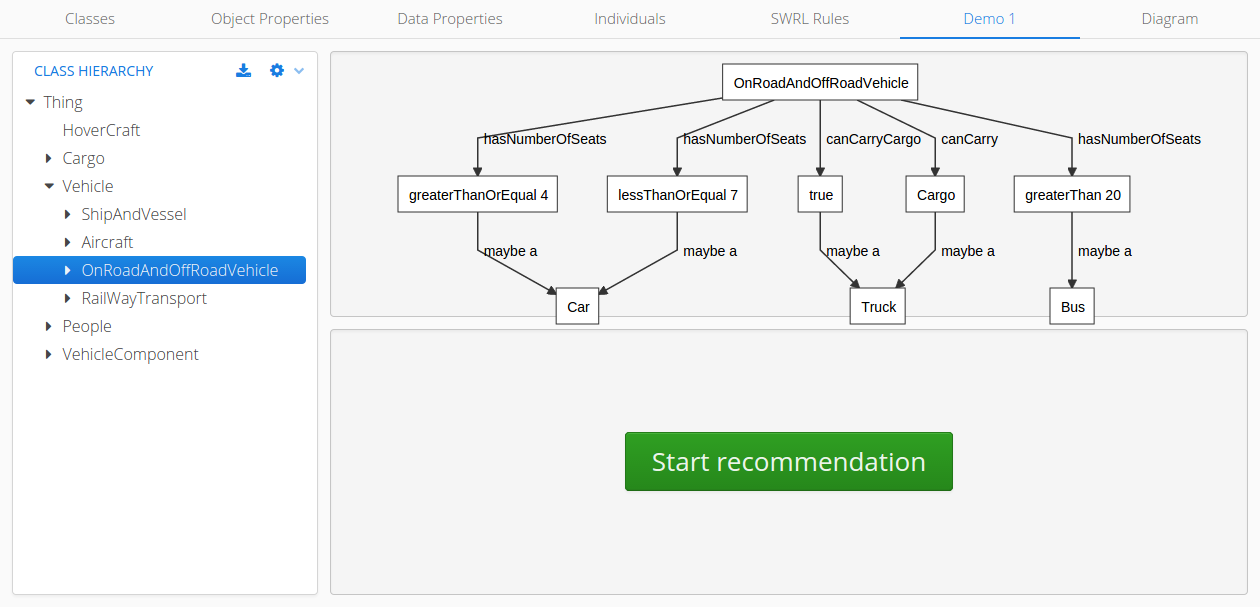
\includegraphics[width=145mm]{Figures/owleditor_demoSheet.png}}
	\caption{Demo Tab trong UIT-OWL Editor\label{overflow}}
\end{figure}
Demo Tab không nằm trong thành phần tiêu chuẩn mà một Ontology Editor bắt buộc phải có như các Tab đã giới thiệu. Tuy nhiên, chúng em xây dựng Demo Tab trong ứng dụng này với mục đích thử nghiệm tính năng hỗ trợ phân loại (sẽ được đề cập trong phần sau của chương này). Các thành phần của tab này gồm:
\begin{enumerate}
\item Panel bên trái phía trên là ClassHierachicalPanel có một cấu trúc dạng cây với các node chính là các lớp nằm trong OWL2 Ontology, với các chức năng thêm/xóa Sub/Sibling Class. Khi chọn một lớp ở đây thì ListSelect ở bên dưới sẽ hiển thị một danh sách cá thể thuộc lớp này.
\item Panel bên trái phía dưới là IndividualList hiển thị một danh sách gồm các cá thể thuộc lớp được chọn ở trên, có các tính năng thêm/xóa cá thể.
\item Panel phía trên bên phải sẽ hiện thị một sơ đồ thể hiện gợi ý phân loại lớp mà cá thể được chọn đang là thành viên.
\item Panel bên phải phía dưới dùng để điền thêm vào các phát biểu cho cá thể dựa theo sơ đồ ở trên.
\end{enumerate}
% Demo Sheet


\section{OWLEditorKit}
\begin{description}
\item[Interface:] \verb|vn.edu.uit.owleditor.OWLEditorKit|
\item[Class implementation:] \verb|vn.edu.uit.owleditor.OWLEditorKitImpl|
\end{description}
Đây là thành quan trọng nhất của toàn bộ ứng dụng đảm nhiệm việc khai thác các API từ OWL-API, nạp/tạo Ontology từ IRI, suy luận, giải thích các phát biểu, parse các chuỗi viết theo cú pháp \textit{Manchester} thành các mô tả lớp và dữ liệu. Thực ra, các chứng năng vừa kể trên hầu hết đều được thực thi nhờ các API của OWL-API, \textit{OWLEditorKit} đóng gói tất cả lại thành một đối tượng để dễ dàng sử dụng trong các UI Component hơn, cũng như tránh việc phải khởi tạo nhiều lần các API.
\subsection{Các chức năng của OWLEditorKit}

\subsubsection{Load Ontology}
Tương ứng với hàm \textit{loadOntologyFromOntologyDocument}, load các tài liệu OWL2 từ tham số là đối tượng \textit{IRI} của OWL-API, ontology khi load xong sẽ được gán cho đối tượng Active Ontology (sẽ được đề cập ngay sau).
\begin{verbatim}
OWLEditor kit = new OWLEditorKitImpl();
kit.loadOntologyFromOntologyDocument(IRI.create("some url"));
\end{verbatim}
\subsubsection{Giải thích các phát biểu trong OWL2 Ontology}
Tương ứng với hàm \textit{explain}, tham số nhận vào là một phát biểu tương đương đối tượng \textit{OWLAxiom} trong OWL-API. Kết quả trả về là một đối tượng \textit{ExplanationTree} chứa các phát biểu giải thích.

\subsubsection{Xóa các thực thể (Entities) trong OWL2 Ontology}
Xóa các phát biểu trong OWL 2 Ontology không phải là một tác vụ dễ dàng vì một phát biểu có thể được sử dụng để xây dựng nên phát biểu khác. Ví dụ:
\begin{verbatim}
Declaration( Class( A ))
SubClassOf(A B)
EquivalentClasses(A C D)
\end{verbatim}
Giả sử chúng ta muốn xóa phát biểu \textit{Declaration( Class( A ))} thì \textbf{bắt buộc} chúng ta phải xóa luôn những phát biểu có liên quan đến A là \textit{SubClassOf và EquivalentClasses} bởi vì nếu không có phát biểu khẳng định sự tồn tại của A thì những phát biểu còn lại sẽ trở nên vô nghĩa. Tuy nhiên để thực hiện tác vụ này OWL-API cung cấp cho chúng ta một đối tượng là \textit{OWLEntityRemover} với tính năng duyệt qua mọi phát biểu có liên quan đến thực thể cần xóa, xóa tất cả các phát biểu đó trước khi xóa thực thể. Đối tượng này được sử dụng qua getter \textit{getEntityRemover}.

\subsubsection{Nhà máy sản xuất ra mọi loại đối tượng trong OWL 2 Ontology}
Một chức năng thực sự hữu ích được khai thác từ đối tượng \textit{OWLDataFactory} của OWL-API, với số lượng đối tượng (thực thể, mô tả lớp, thuộc tính, phát biểu, ...) rất lớn đã đề cập ở chương 2, rất khó để chúng ta có thể nhớ và sử dụng chúng dễ dàng. \textit{OWLDataFactory} cung cơ chế để tạo ra mọi loại phát biểu trong OWL 2 Ontology một cách tiện lợi. Ví dụ như:
\begin{verbatim}
// Declaration( NamedIndividual(a:Peter) )
OWLNamedIndividual Peter = factory.getOWLNameIndividual("a:Peter");
// Declaration( DataProperty(a:HasAge) )
OWLDataProperty hasAge = factory.getOWLDataProperty("a:HasAge");
// ClassAssertion( a:Person a:Peter )
OWLLiteral age = factory.getOWLLiteral(22);
\end{verbatim}
Trong \textit{OWLEditorKit}, \textit{OWLDataFactory} được truy xuất qua getter \textit{getOWLDataFactory()}.

\subsubsection{Nhà máy sản xuất ra mọi loại đối tượng dữ liệu cho ứng dụng UIT-OWL Editor}
{\let\thefootnote\relax\footnotetext{
		*: \textit{http://en.wikipedia.org/wiki/Factory\_method\_pattern}}
}
\begin{description}
\item[Interface:] \verb|vn.edu.uit.owleditor.data.OWLEditorDataFactory|
\item[Class Implementation:] \verb|vn.edu.uit.owleditor.data.OWLEditorDataFactoryImpl|
\end{description}
Học tập mô hình \textit{Factory Pattern} \textsuperscript{*} từ đối tượng \textit{OWLDataFactory}, chúng em cũng tự xây dựng một đối tượng với mục tiêu là cung cấp một cơ chế tiện lợi để tạo ra các đối tượng dữ liệu và các event trong UIT-OWL Editor. Tham số khởi tạo của \textit{OWLEditorDataFactory} chính là \textit{OWLEditorKit}. Ví dụ để tạo sự kiện thêm một phát biểu về lớp vào Ontology:
\begin{verbatim}
OWLClass person, man; // Tạo sự kiện thêm phát biểu về lớp
OWLEditorEvent.ClassAxiomAdded event =
   owlEditorDataFactory.getSubClassOfAddEvent(man, person);
\end{verbatim}

\subsubsection{Parse chuỗi thành các mô tả lớp (OWLClassExpression)}
OWLEditorKit cũng được tích hợp một đối tượng \textit{ManchesterOWLSyntaxParser} trong OWL-API, nhiệm vụ là để parse các đoạn text từ người dùng theo cú pháp \textit{Manchester} thành các mô tả lớp (OWLClassExpression) hay các miền dữ liệu (OWLDataRange). Parser này được sử dụng thông qua getter \textit{getParser} hoặc parse trực tiếp qua hàm \textit{parseClassExpression(String stringToParse)} . Ví dụ:
\begin{verbatim}
OWLEditorKit eKit = new OWLEditorKitImpl(); // nạp ontology ...
OWLClassExpression ce2 = eKit.parseClassExpression("Has some Kid");
\end{verbatim}

\subsubsection{Suy luận các phát biểu}
Tính năng suy luận được đáp ứng bởi Pellet Reasoner đề cập ở chương trước. Reasoner cũng đã được tạo sẵn trong \textit{OWLEditorKitImpl}, truy cập thông qua getter \textit{getReasoner()} và sử dụng như mô tả ở chương trước.

\subsubsection{Áp dụng các thay đổi về phát biểu cho ontology}
Chức năng này được thực thi bởi đối tượng \textit{OWLOntologyManager} được khởi tạo cùng với lớp \textit{OWLEditorKitImpl}, sử dụng thông qua getter \textit{getModelManager()}.
\textit{OWLOntologyManager} sẽ được sử dụng để áp dụng thay đổi trong các hàm Subscriber (sẽ được đề cập trong phần Xử lý sự kiện).

\subsection{Một số đối tượng đáng chú ý khác trong OWLEditorKitImpl}
Ngoài các chức năng đi kèm với các đối tượng quan trong kể trên trong implementation của \textit{OWLEditorKit} cũng có một số đối tượng mà chúng ta cũng cần phải lưu ý.
\subsubsection{Active Ontology}
Biến  \textit{activeOntology} là một đối tượng \textit{OWLOntology} của OWL-API được khai báo trong \textit{OWLEditorKitImpl}. Biến này chính là OWL2 Ontology hiện hành đang được thao tác trên giao diện. Các thao tác thêm/xóa/sửa các phát biểu qua các giao diện đều sẽ được cập nhật và áp dụng lên đối tượng \textit{OWLOntology} này.
\subsubsection{Manchester Renderer}
Hàm static \textit{OWLEditorKitImpl.render(OWLObject)} dùng render hay chuyển đổi các đối tượng OWL 2 thành dạng chuỗi (cú pháp Manchester), chủ yếu để render các phát biểu, mô tả lớp/thuộc tính/kiểu dữ liệu.
\subsubsection{Lấy tên thực thể}
Hàm static \textit{OWLEditorKitImpl.getShortForm(OWLEntity)} dùng lấy tên các đối tượng \textit{OWLEntity}. Ví dụ: \textit{longIRI:Person} -> \textit{Person}


\section{Xử lý sự kiện trong UIT-OWL Editor}
{\let\thefootnote\relax\footnotetext{
		*: \textit{http://en.wikipedia.org/wiki/Publish\%E2\%80\%93subscribe\_pattern}}
}
Để xử lý các sự kiện trong ứng dụng, chúng em sử dụng thư viện Guava EventBus \cite{guava}. \textit{EventBus} cho phép giao tiếp theo kiểu công bố và theo dõi (\textit{publish-subscribe}\textsuperscript{*}), các UI Component không cần thiết phải khai báo với nhau (để biết được tồn tại của nhau). Thư viện được được thiết kế nhằm thay thế kiểu giao tiếp chia sẻ sự kiện trong tiến trình (in-process event distribution) bằng cách khai báo rõ ràng các thành phần có liên quan tới sự kiện với nhau (khai báo đối tượng tạo ra sự kiện, đối tượng sẽ lắng nghe sự kiện với nhau). Cơ chế xử lý sự kiện này của ứng dụng có thể được miêu tả trong hình sau:
\begin{figure}[h!]
	\centering
	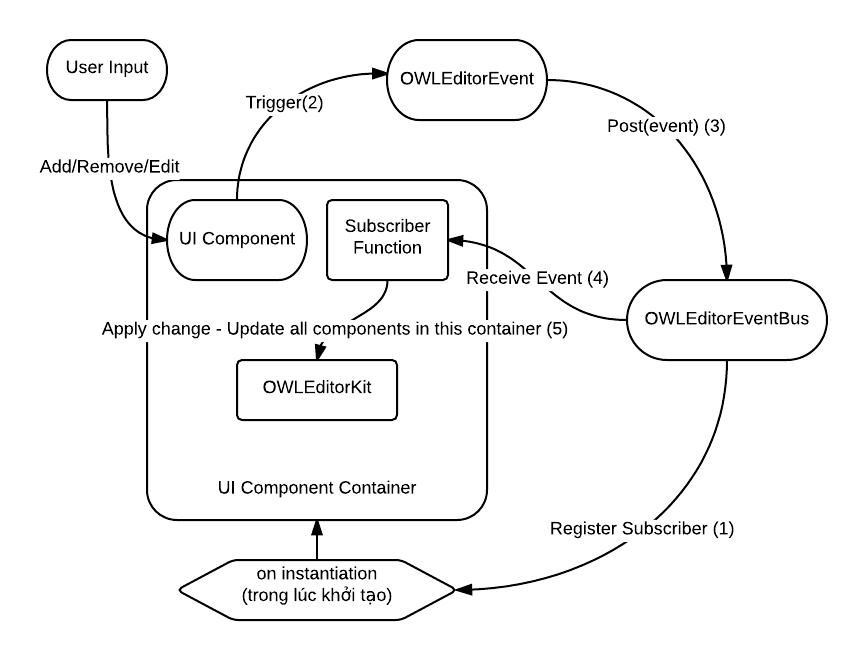
\includegraphics[width=145mm]{Figures/owleditor_eventBus.png}
	\caption{Xử lý sự kiện trong UIT-OWL Editor\label{overflow}}
\end{figure}
Để hiểu rõ hơn nữa, chúng em xin được lấy sự kiện thêm một phát biểu \textit{SubClassOf} trong Panel có tên tương ứng nằm trong Tab "Classes". Panel này là một đối tượng lớp \textit{ClassPanel} nằm trong \textit{ClassExpressionPanelContainer} và các chức năng \textit{EventBus} của toàn ứng dụng có thể được sử dụng qua lớp \textit{OWLEditorEventBus}. 
\begin{verbatim}
class ClassExpressionPanelContainer extends AbstractPanelContainer {
    ClassPanel subClsPanel; 
    public ClassExpressionPanelContainer {
       subClsPanel = new ClassPanel("SubClass Of: ") {
          void initActionADD() { 
          // Mở một cửa số nhỏ để nhập mô tả lớp mới vào
          UI.getCurrent()
            .addWindow(new buildAddClassExpressionWindow(...));            
             ...
          }
       }
       this.addComponent(subClsPanel); 
	   OWLEditorEventBus.register(this); // Bước 1 trong sơ đồ
    }
    ...
    // Annotation @Subscribe được cung cấp bởi thư viện EventBus
    // Bước 4 trong sơ đồ 
    @Subscribe 
    public void handlAxiomAdd(OWLEditorEvent.ClassAxiomAdded event) {
       // Bước 5 trong sơ đồ
       OWLEditorKit kit = OWLEditorUI.getEditorKit();
       kit.getModelManager.applyChange(new 
           AddAxiom(kit.getActiveOntology(),event.getAxiom));
	       // render các thay đổi lên các UI Components
    }  
}
class buildAddClassExpressionWindow extends ... {
    ...
    // sự kiện khi nhấn save tương ứng bước 2 trong sơ đồ
    Button.ClickListener initSaveListener() {
       return click -> {
          OWLClassExpression ce = editorKit
            .parseClassExpression("some value from Textfield");
          // tương ứng bước 3 
          OWLEditorEventBus.post(ClassAxiomAdded(.., ce));
       }
    }
}
\end{verbatim}
Hình sau miêu tả lại thao tác người dùng trên UI:
\begin{figure}[h!]
	\centering
	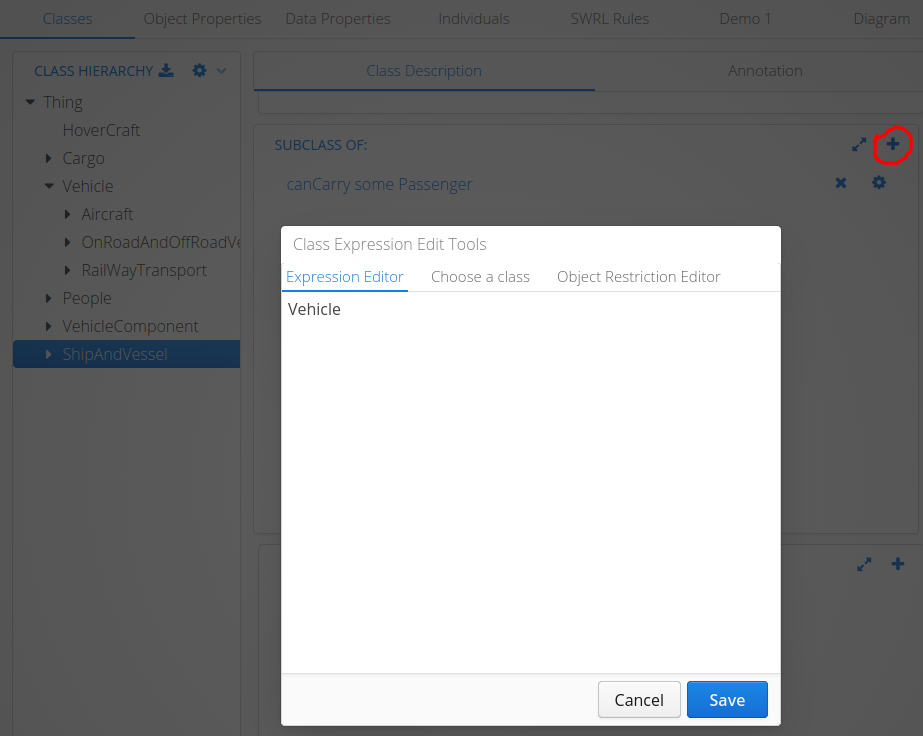
\includegraphics[width=145mm]{Figures/eventBusExplain.png}
	\caption{Xử lý sự kiện trong UIT-OWL Editor\label{overflow}}
\end{figure}
Đầu tiên trước khai mọi sự kiện diễn ra một \textit{Subscriber} cần được đăng ký trong một Component nào đó bằng Annotation @Subscribe và method \textit{register} (đăng ký đây sẽ là listener/subscriber để theo dõi các sự kiện tương ứng). Khi người dùng, nhấn dấu cộng ở góc của Panel \textit{SubClassOf} sẽ mở ra một cửa sổ để nhập vào mô tả lớp, nút save được bấm thì cũng là lúc mà sự kiện được công bố (publish) lên \textit{EventBus} (qua phương thức \textit{post} ở bước 3), do đã đăng ký trước nên phương thức \textit{Subscribe} sẽ được EventBus truyền cho đúng kiểu event mà nó đang theo dõi. Lưu ý: phương thức nào làm Subscriber thì bắt buộc phải có một tham số duy nhất là sự kiện với kiểu tương ứng với nơi mà sự kiện đó được công bố, đồng thời access-level của phương thức phải là public.
\\
Như đã trình bày, nguyên tắc của EventBus để phân biệt các sự kiện chỉ là kiểu của nó. Chính vì thế mà với mỗi loại hành động thêm/xóa/sửa trên loại thực thể, hoặc phát biểu của thực thể sẽ có một loại sự kiện tương ứng. Ví dụ: đối với các phát biểu liên quan tới lớp sẽ có 3 loại tương ứng là ClassAxiomAdded, ClassAxiomRemoved và ClassAxiomEdit. Tương tự cho các thực thể và phát biểu còn lại. Chi tiết hơn, thầy cô và bạn đọc có thể tham khảo thêm trong lớp \textit{vn.edu.uit.owleditor.event.OWLEdtiorEvent} trong mã nguồn của ứng dụng \cite{owleditorSrc}.


\section{Tổ chức các đối tượng dữ liệu - Data Model}
Đã được đề cập trong lúc giới thiệu về Vaadin, Data Model trong Vaadin được chia làm 3 cấp từ thấp đến cao Property, Item và Container. Trong ứng dụng, chúng em chỉ sử dụng 2 dạng data model là Property và Container. 
\subsection{HierarchicalContainer}
%Vaadin cung cấp một lớp gọi là \textit{HierarchicalContainer} chuyên dùng để chứa dạng dữ liệu có cấu trúc phân cấp. Qua giới thiệu ở chương 2, chúng ta đã biết rằng các t đều là những đối tượng có quan hệ SubClassOf, SubObjectPropertyOf và SubDataPropertyOf hay có thể nói 3 thực thể kể trên có cấu trúc phân cấp.
\begin{figure}[ht!]
	\centering
	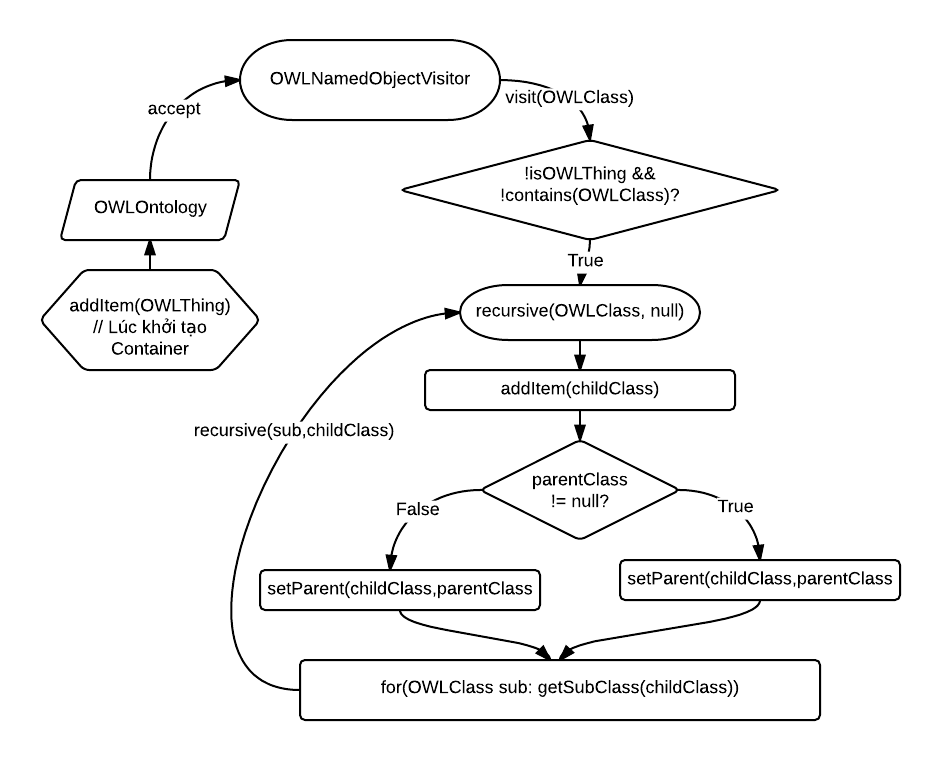
\includegraphics[width=145mm]{Figures/owleditor_hccontainer.png}
	\caption{OWLClassHierarchicalContainer trong UIT-OWL Editor\label{overflow}}
\end{figure}
Để thể hiện tính chất phân cấp của các thực thể như lớp, thuộc tính đối tượng và dữ liệu trong OWL 2 Ontology, chúng ta có thể dùng Tree Component của Vaadin. Tuy nhiên, với việc UI Component Tree được sử dụng lặp lại nhiều lần trong ứng dụng, nên việc tách biệt các đối tượng dữ liệu với UI đã sẽ giúp chúng ta tiết kiệm được những khai báo lại không cần thiết, dữ liệu thay đổi trong DataModel cũng sẽ được cập nhật đến toàn bộ những UI Component mà nó được sử dụng (binding). Để hiểu rõ hơn về cách tổ chức của \textit{HierarchicalContainer} chúng em xin được lấy  \textit{AbstractOWLObjectHierarchicalContainer}, được thừa kế bởi \textit{HierarchicalContainer} của lớp, thuộc tính đối tượng và dữ liệu. Nó gồm những đặc điểm quan trọng sau:
\begin{itemize}
	
\item Thừa kế từ HierarachicalContainer của Vaadin nên sẽ có sẵn các phương thức \textit{addItem}, \textit{setParent} phục vụ cho việc thêm, và sắp xếp item theo cấu trúc cây.
\item Gồm một \textit{OWLEntityRemover} dùng để xóa thực thể (OWLEntity) khi nhận yêu cầu xóa từ UI Component.
\item Gốm một đối tượng OWLNamedObjectVisitor (xem lại Visitor Pattern ở chương trước) có chức năng tìm đóng loại cá thể, sau đó thêm chúng vào HierachicalContainer.
\item Gồm một \textit{OWLOntologyChangeVisitor} dùng để cập nhật sự thay đổi trong container cho đồng bộ với sự thay đổi của OWLOntology khi thêm/xóa các thực thể và phát biểu SubClass/SubPropertyOf.
\item Gồm một hàm đệ quy với mục đích là sắp xếp các item trong HierarchicalContainer cho đúng với sự phân cấp của chúng trong OWL2 Ontology.
\end{itemize}
Dưới đây là sơ đồ mô tả lại giải thuật thêm và sắp xếp các item lên cấu trúc cây của \textit{OWLClassHierarchicalContainer} thừa kế từ lớp Abstract ở trên. Chú thích: \textit{contains} là một hàm nhằm xác định đối tượng được xét đã tồn tại trong Container chưa.

\subsection{List}
Đây thật ra là lớp mà HierarchicalContainer trong Vaadin thừa kế IndexedContainer, mục đích của Container dạng này là dùng để chứa các item theo dạng danh sách, chúng em sử dụng chúng để chứa các đối tượng như OWLNamedIndividual, OWL2Datatype 
\subsection{Property}
Mục đích đưa các đối tượng thành Property của Vaadin cũng tương tự như Container, các đối tượng OWL2 sẽ được sử dụng lại nhiều lần bởi các UI Component sử dụng (binding) nó nên sử dụng Property chứa các đối tượng OWLObject sẽ giúp tiết kiệm những lần truyền tham số (là các OWLObject) giữa các UI Component. Các Property trong ứng dụng được đặt tên theo quy ước \textit{OWL} + tên thành phần OWL 2 + \textit{Source}. Ví dụ
\begin{verbatim}
OWLClass -> OWLCLassSource
OWLClassExpression -> OWLClassExpressionSource
\end{verbatim}

\subsection{Converter}
Trong ứng dụng chúng em có sử dụng một số Converter tự định nghĩa vốn được xây dựng từ interface Converter (đã trình bày trong phần giới thiệu Vaadin Framework) với mục đích chuyển đổi các thực thể gồm lớp, thuộc tính đối tượng, thuộc tính dữ liệu và cá thể có tên. Mục tiêu xây dựng các Converter này là sẽ giúp chuyển đối giữ chuỗi sang đối tượng tương ứng là OWLClass, OWLObjectProperty, OWLDataProperty và OWLNamedIndividual một cách nhanh chóng khi thêm các cá thể mới. Chi tiết hơn có thể xem package \textit{vn.edu.uit.owleditor.utils.converter} \cite{owleditorSrc}.

\section{Các tính năng nổi bật của UIT-OWL Editor}
Ngoài những tính năng đã trình bày sơ qua trong phần đầu UI, phần này chúng em xin dành để liệt kê ra một số tính năng nổi bật trong ứng dụng.

\subsection{Trình biên tập các mô tả lớp}
Trình biên tập cho phép nhập các chuỗi các khai báo về mô tả lớp (class expression) theo cú pháp Manchester, trình biên tập mô tả lớp cũng được tích hợp một danh sách autocomplete gồm các thực thể đã được khai báo trong ontology. Mỗi loại cá thể trong danh sách autocomplete sẽ được hiện thị theo một Icon khác nhau tương ứng với chữ cái đầu tiên của loại đó như \textbf{O} cho ObjectProperty, \textbf{C} cho Class, \textbf{D} cho DataProperty và \textbf{I} cho NamedIndividual. Khi nhấn nút save, ứng dụng sẽ tự động parse chuỗi thành Đối tượng OWLClassExpression bằng ManchesterSyntaxParser trong OWLEditorKit, sẽ có thông báo lỗi nếu nhập sai cú pháp.
\begin{figure}[h!]
	\centering
	\frame{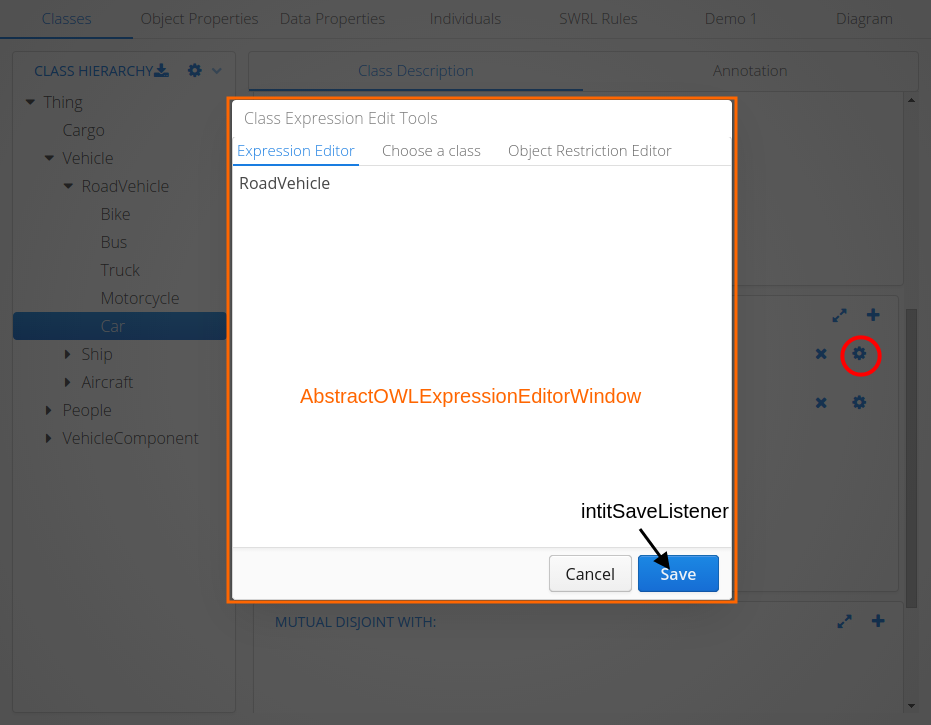
\includegraphics[width=145mm]{Figures/owleditor_ceeditor.png}}
	\caption{Biên tập mô tả lớp trong UIT-OWL Editor\label{overflow}}
\end{figure}
\\
Lý do chọn Manchester Syntax vì chúng em ưu tiên cú pháp thân thiện, gần với ngôn ngữ con người hay sử dụng hàng ngày (thầy cô và bạn đọc có thể xem lại trong chương giới thiệu về OWL 2).
\subsection{Trình biên tập SWRL Rule}
Trình biên tập cho phép biên tập SWRL Rule bằng cú pháp được giới thiệu trong chương \textit{Semantic Web Rule Language}, tổ chức các Rule theo tên, và thêm giải thích cho Rule.
\begin{figure}[h!]
	\centering
	\frame{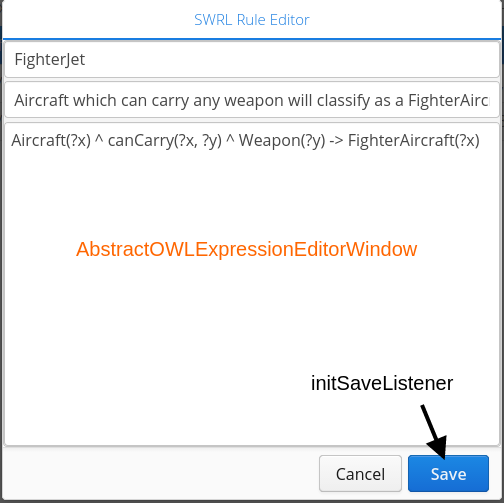
\includegraphics[width=145mm]{Figures/owleditor_ruleeditor.png}}
	\caption{Biên tập SWRL Rule trong UIT-OWL Editor\label{overflow}}
\end{figure}
Trình biện tập rule được đảm nhiệm bởi thành phần \textit{SWRLAPIRuleOntology} trong \textit{OWLEditorKit} đã được giới thiệu ở trên.

\subsection{Tính năng suy luận - Reasoning}
Để sử dụng tính năng suy luận, chúng ta chọn biểu tượng bánh răng ở góc phải của Panel chứa cây các lớp trong Ontology, sẽ mở ra một menu với tùy chọn "Start reasoner". Hãy chọn nó, chương trình sẽ thông báo "Reasoner Activated". Đối với Tab \textit{Individual}, chọn bất kì một lớp nào trong cây rồi chọn một trong các cá thể của lớp đó, các phát biểu có liên quan đến cá thể đó sẽ hiển thị các panel nhỏ tương ứng với các loại phát biểu của cá thể.
\begin{figure}[h!]
	\centering
	\frame{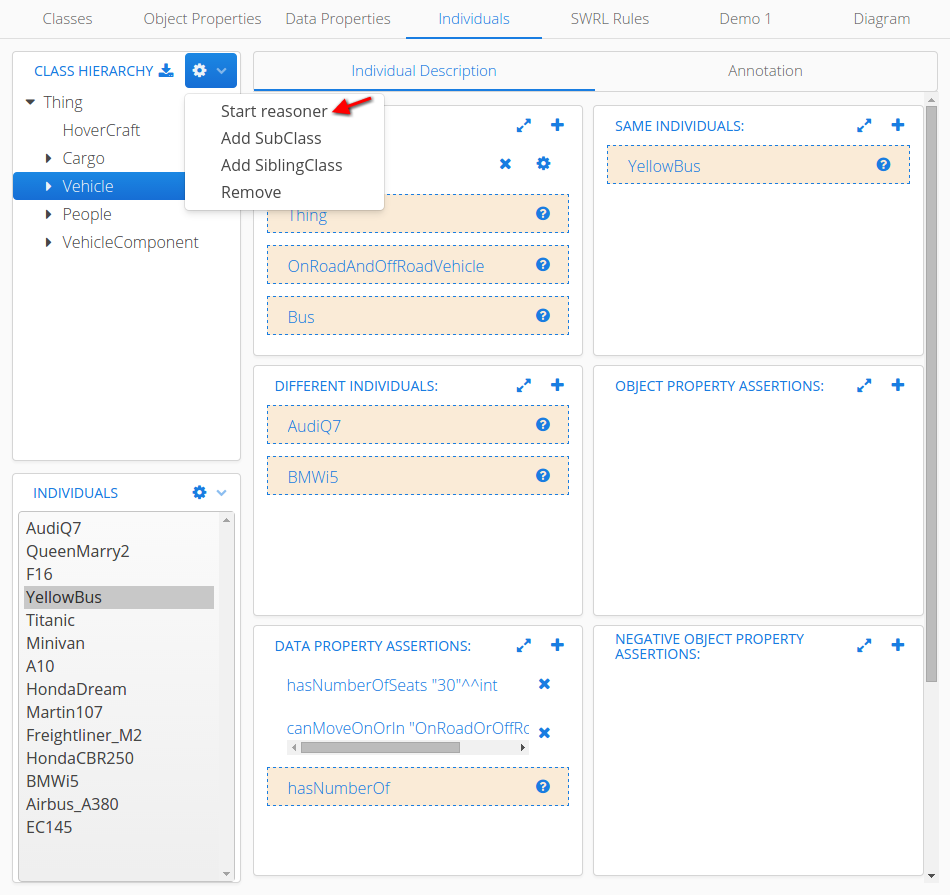
\includegraphics[width=145mm]{Figures/owleditor_reasoning.png}}
	\caption{Tính năng suy luận trong UIT-OWL Editor\label{overflow}}
\end{figure}
Trong hình, các phát biểu được tô đậm chính là các phát biểu được suy luận ra từ Ontology nhờ Pellet Reasoner. Để xem giải thích tại sao cho các phát biểu này chúng ta chọn biểu tượng ? ở cuối mỗi phát biểu. Ví dụ để xem tại sao cá thể \textit{AudiQ7} lại được phân loại thuộc lớp \textit{Car} chúng ta chọn biểu tượng ? ở cuối phát biểu \textit{"Car"}.
\begin{figure}[H]
	\centering
	\frame{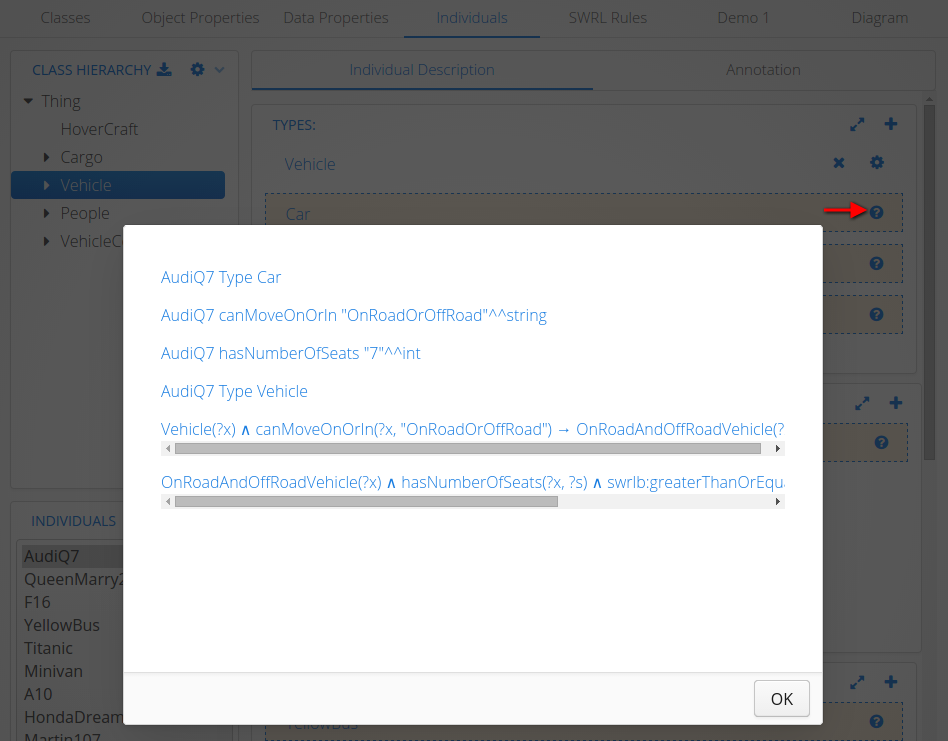
\includegraphics[width=145mm]{Figures/owleditor_explanationWindow.png}}
	\caption{Giải thích suy luận trong UIT-OWL Editor\label{overflow}}
\end{figure}
Việc giải thích được đảm nhiệm bởi đối tượng \textit{DefaultExplanationGenerator} của OWL-API hoạt động theo nguyên lý được mô tả ở chương \textit{"Tính nhất quán của Ontology"}.

\section{Tính năng hỗ trợ phân loại - Demo Tab}
\begin{figure}[ht!]
	\centering
	\frame{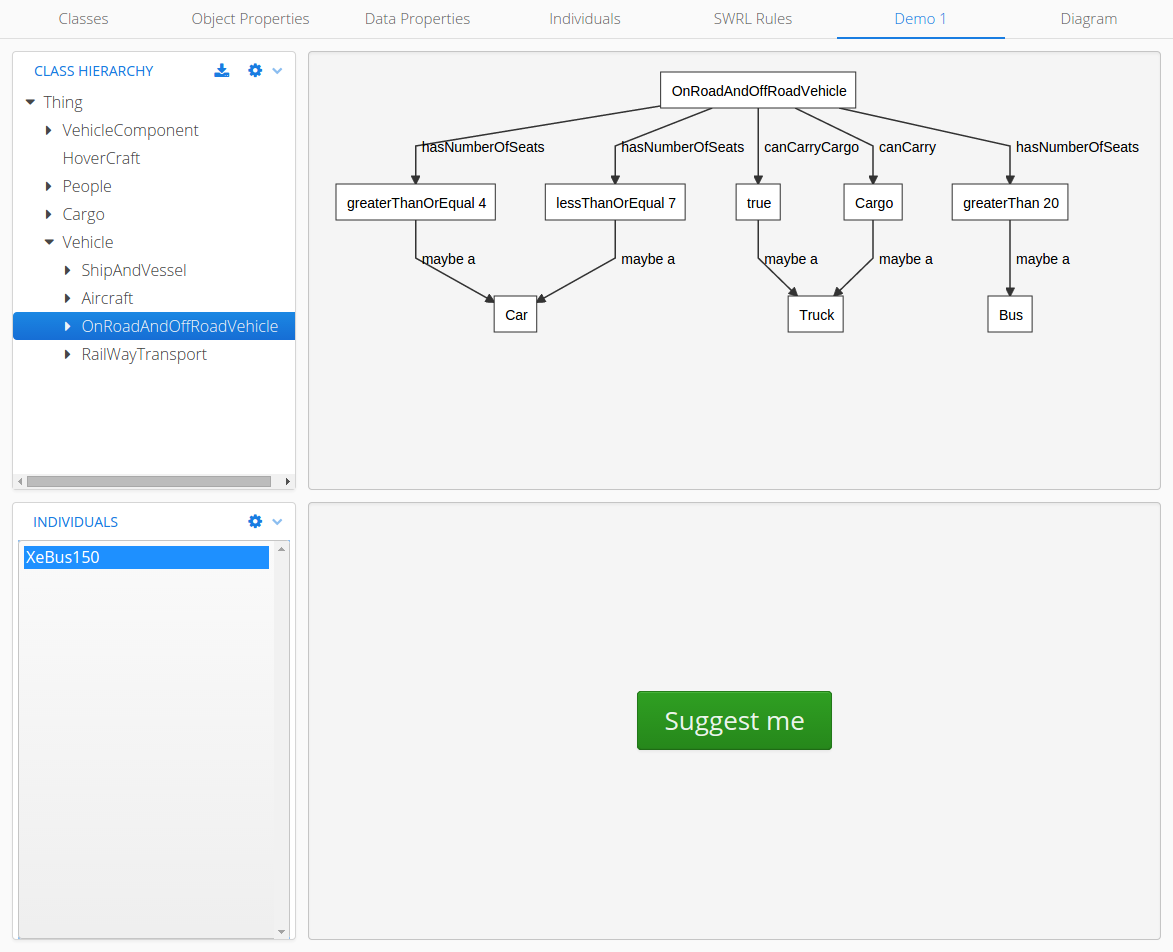
\includegraphics[width=145mm]{Figures/owleditor_demo1.png}}
	\caption{Tính năng hỗ trợ phân loại trong UIT-OWL Editor (phần 1)\label{overflow}}
\end{figure}
Việc sử dụng SWRL Rule hay đơn giản hơn là đọc và hiểu ý nghĩa có nó thường rất khó đối với người dùng thông thường, chưa kể đến việc chưa có cơ chế tổ chức các SWRL rule một cách khoa học, sẽ có những trường hợp chúng ta vô tình tạo ra những điều kiện trùng nhau dẫn đến 2 kết quả khác nhau hoặc ngược lại. Hiểu được nhược điểm này của SWRL Rule, chúng em đã thiết kế thêm tính năng hỗ trợ phân loại với giao diện là Tab Demo trong ứng dụng, với khả năng vẽ ra một sơ đồ dựa theo chuỗi các điều kiện - kết quả có liên quan đến lớp đang chứa cá thể được chọn để phân loại. Để minh họa cho tính năng này ,chúng em xin trích một đoạn chứa các SWRLRule trong ontology \textit{Transport.owl} \cite{owleditorSrc} (được chúng em xây dựng để làm demo cho tính năng phân loại). Hình trên mô tả lại các rule sau:
\begin{verbatim}
# Phương tiện đường bộ có thể chở hàng hóa (Cargo) là xe tải (Truck)
OnRoadAndOffRoadVehicle(?x) ^ canCarry(?x, ?y) ^ Cargo(?y)  -> Truck(?x)
# Phương tiện đường bộ có khả năng chở hàng là xe tải (Truck)
OnRoadAndOffRoadVehicle(?x) ^ canCarryCargo(?x, true) -> Truck(?x)
# Phương tiện đường bộ có số 4 <= chỗ ngồi <= 7 là xe hơi (Car)
OnRoadAndOffRoadVehicle(?x) ^ hasNumberOfSeats(?x, ?s)
                            ^ swrlb:greaterThanOrEqual(?s, 4) 
                            ^ swrlb:lessThanOrEqual(?s, 7)  -> Car(?x)
# Phương tiện đường bộ có số chỗ ngồi >= 20 là xe Bus 
OnRoadAndOffRoadVehicle(?x) ^ hasNumberOfSeats(?x, ?s) 
                            ^ swrlb:greaterThan(?s,20) -> Bus(?x)                               
\end{verbatim}
Trong hình chỉ miêu tả những rule nào có liên quan đến lớp \textit{OnRoadAndOffRoadVehicle} vốn là lớp chứa cá thể \textit{XeBus150} trong hình, làm vậy để hạn chế những thông tin không cần thiết đối với người dùng. Khi chọn \textit{Suggest Me} sẽ tạo ra một loại các UI Component phục vụ để tạo ra các phát biểu về cá thể \textit{XeBus150}.
\begin{figure}[h!]
	\centering
	\frame{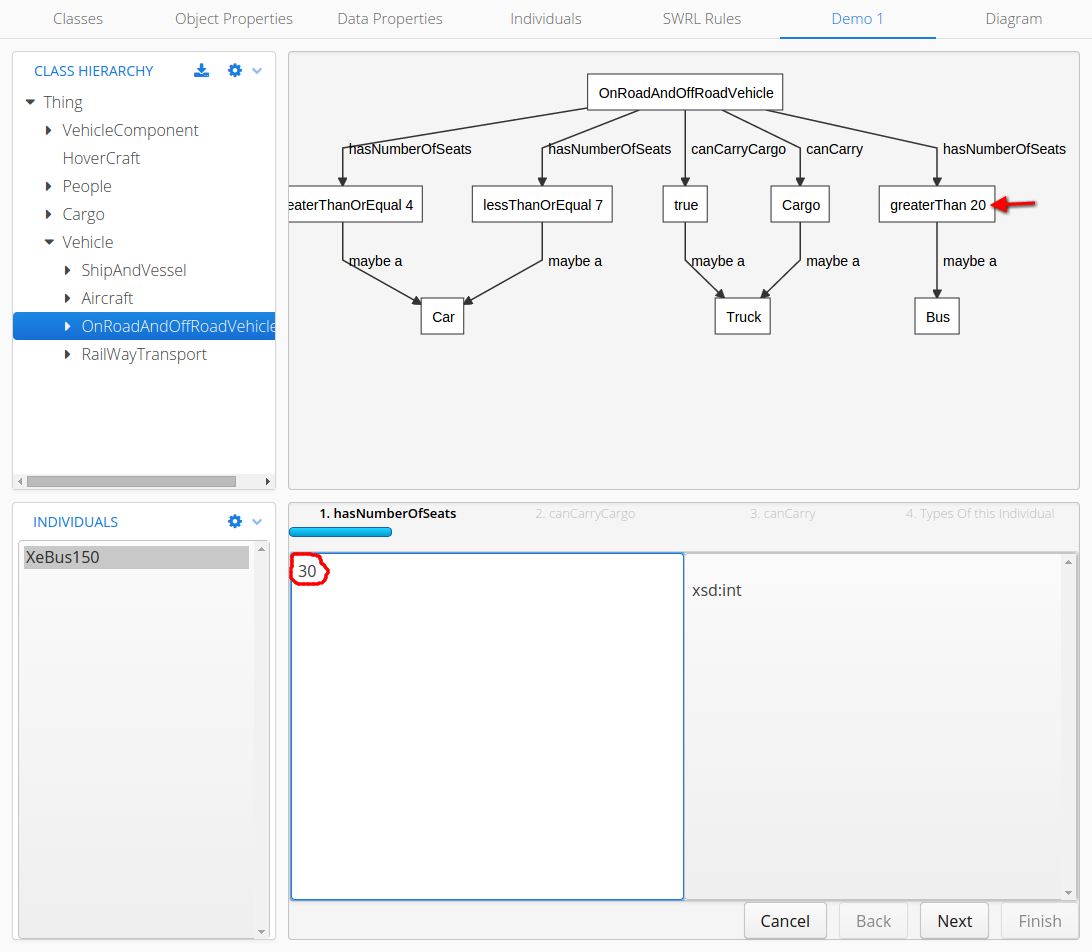
\includegraphics[width=145mm]{Figures/owleditor_demo2.png}}
	\caption{Tính năng hỗ trợ phân loại trong UIT-OWL Editor (phần 2)\label{overflow}}
\end{figure}
\begin{figure}[h!]
	\centering
	\frame{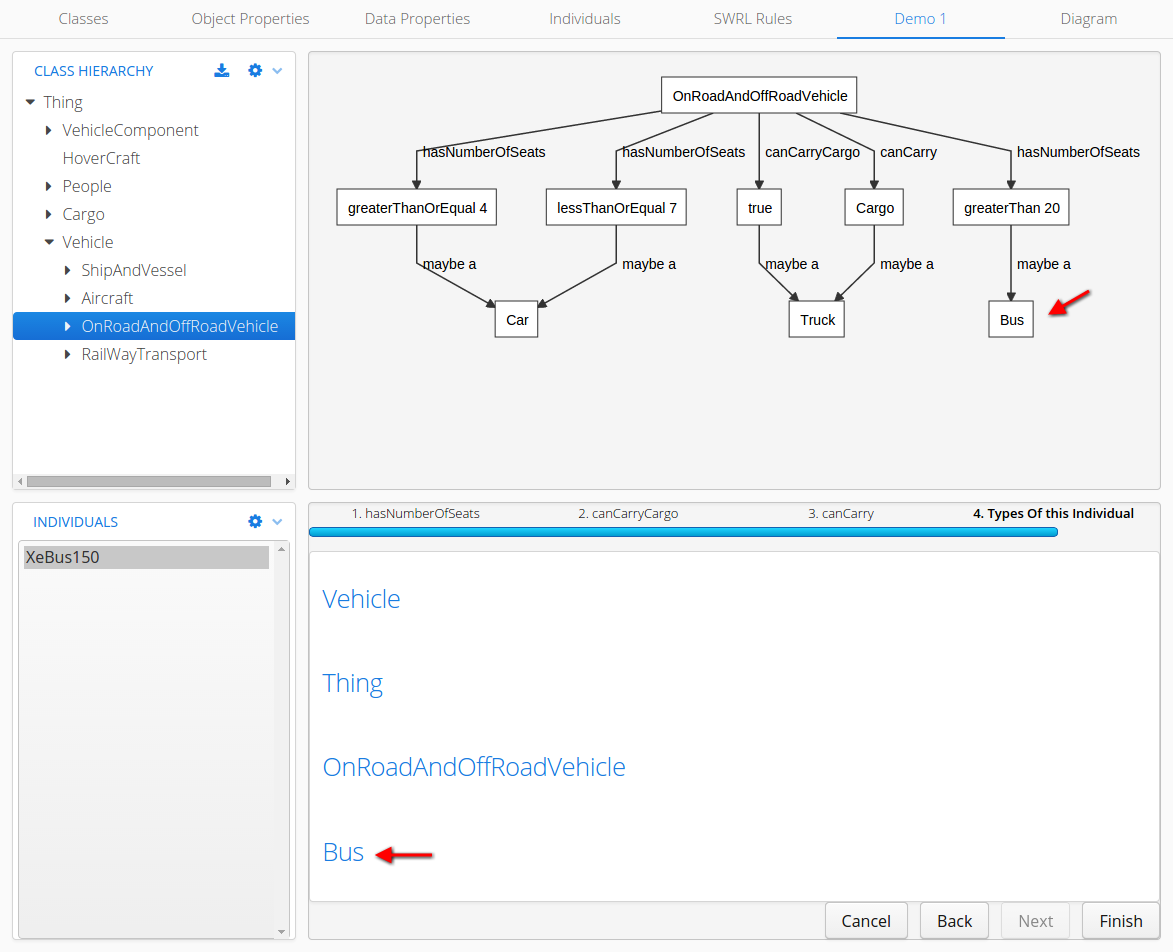
\includegraphics[width=145mm]{Figures/owleditor_demo3.png}}
	\caption{Tính năng hỗ trợ phân loại trong UIT-OWL Editor (phần 3)\label{overflow}}
\end{figure}
Trong hình trên mỗi bước sẽ tương ứng với những phát biểu có liên quan đến \textit{OnRoadAndOffRoadVehicle} như trong sơ đồ. Miền dữ liệu (Range) của thuộc tính dữ liệu và thuộc tính đối tượng cũng sẽ được áp dụng nhằm giảm bớt những thông tin không cần thiết, thuộc tính \textit{hasNumberOfSeats} có DataPropertyRange( xsd:int) nên ở cột bên phải chúng ta chỉ thấy kiểu dữ liệu này thay vì là một loạt kiểu dữ liệu như xsd:string, xsd:byte, v.v... . Khi đến bước cuối cùng, reasoner sẽ đánh giá lại các thông tin mà chúng ta vừa nhập vào ở các bước trước để đưa kết quả phân loại phù hợp như đã được biểu diễn trong sơ đồ.

\section{Xây dựng một ontology để trình bày quá trình phân loại}
\textbf{Giới thiệu} Transport.owl là một ontology do nhóm tự xây dựng nên, đối tượng chủ yếu là các phương tiện giao thông đường bộ, đường thuỷ, đường hàng không, bên cạnh đó là các bộ phận của phương tiện như động cơ, hệ thống rô-tơ,... các đối tượng liên quan như hàng hoá, hành khách, bộ phận của phương tiện, ... .
Ontology được xây dựng phục vụ nhu cầu demo hệ thống phân loại tự động, nên có một vài điểm không bám sát theo đúng với thực tế.
\subsection{Các lớp trong transport.owl (không bao gồm OWL Thing)}
\begin{itemize}
\item Lớp Cargo : hàng hoá
\item Lớp Vehicle: phương tiện
		\begin{itemize}
		\item Lớp ShipAndVessel : phương tiện đường thuỷ
			\begin{itemize}
			\item Lớp Boat : thuyền
			\item Lớp Vessel
			\item Lớp Cruiser
			\end{itemize}
		\item Lớp Aircraft : phương tiện đường hàng không
			\begin{itemize}
			\item Lớp WingAircraft : máy bay có cánh
			\item Lớp Helicopter : trực thăng 
			\item Lớp FighterAircraft : máy bay chiến đấu
			\item Lớp CargoAircraft : máy bay chở hàng
			\item Lớp PassengerAircraft : máy bay chở khách
			\end{itemize}
		\item Lớp OnRoadAndOffRoadVehicle : phương tiện đường bộ
			\begin{itemize}
				\item Lớp Truck : xe tải
				\item Lớp Bike : xe đạp
				\item Lớp Car : xe hơi
				\item Lớp Motorcycle : xe máy
				\item Lớp Bus : xe bus
			\end{itemize}	
		\item Lớp RailwayTransport : phương tiện đường sắt
			\begin{itemize}
				\item Lớp ExpressTrain
				\item Lớp Metro
			\end{itemize}
		\end{itemize}
\item Lớp People : con người
	\begin{itemize}
	\item Lớp Pilot : phi công
	\item Lớp Passenger : hàng khách
	\item Lớp Driver : tài xế
	\end{itemize}
\item Lớp Vehicle Component : bộ phận của phương tiện
	\begin{itemize}
	\item Lớp Axile
	\item Lớp Body
	\item Lớp Wing : cánh
	\item Lớp Wheel : bánh xe
	\item Lớp RotorSystem : hệ thống rô-tơ
	\item Lớp Engine : động cơ
	\item Lớp Weapon : vũ khí
	\item Lớp Rotor : rô-tơ
	\item Lớp RotorSystem : hệ thống rô-tơ
	\item Lớp Wagon : hàng hoá
	\item Lớp Sprocket
	\end{itemize}
\end{itemize}
\subsection{Các thuộc tính đối tượng trong transport.owl (không bao gồm OWL TopObjectProperty)}
\begin{itemize}
\item hasPart : có bộ phận (là inverse của isPartOf)
\item canBeCarriedBy : có thể được mang bởi đối tượng khác (inverse của canCarry)
\item moveOn : di chuyển được trên
\item isPartOf : là bộ phận của (là inverse của hasPart)
\item canCarry : có thể mang theo (inverse cuả canBeCarriedBy)
\end{itemize}
\subsection{Các thuộc tính dữ liệu trong transport.owl (không bao gồm OWL TopObjectProperty)}
\begin{itemize}
	\item canCarry
	\begin{itemize}
		\item canCarryCargo : có thể mang theo hàng hoá
		\item canCarryPassenger : có thể chở hành khách
	\end{itemize}
	\item canMoveOnOrIn : có thể di chuyển được trên
	\item hasNumberOf
	\begin{itemize}
		\item hasNumberOfRotors : có số rô-tơ
		\item hasNumberOfSeats : có số ghế ngồi
		\item hasNumberOfWings : có số cánh
		\item hasNumberOfWheels : có số bánh xe
	\end{itemize}
	\item canCarryNumberOf
	\begin{itemize}
	\item canCarryNumberOfPassenger : có thể chở được số lượng hành khách
	\item canCarryTheAmountOfCargo : có thể mang theo được số lượng hàng hoá
	\end{itemize}		
\end{itemize}

\paragraph{Kết luận} Qua chương này, chúng em đã trình bày về các tính năng nổi bật mà một trình biên soạn Ontology phải có, đồng thời chúng em cũng đã trình bày về những khả năng phân loại mà ngôn ngữ OWL2, SWRL mang lại qua những tính năng suy luận, giải thích và hỗ trợ phân loại. Ở chương kế và cũng là cuối cùng, chúng em xin dành để tổng hợp lại những kết quả đã làm được, những mặt khó khăn, thuận lợi và những hạn chế còn tồn tại, và hơn nữa là hướng phát triển tương lai của công nghệ này.
